\section{Aufbau}
\label{sec:Aufbau}

Der Aufbau des Versuchs ist in Abbildung \ref{fig:aufbau} dargestellt. Das Licht einer Rubidium-Spektrallampe wird durch einer Sammellinse kollimiert und ein Interferenzfilter lässt nur die gewünschte $D_1$-Linie durch. Das Licht wird zunächst linear und anschließend durch ein $\lambda/4$-Plättchen zirkulär polarisiert.\\
Das rechtszirkular polarisierte Licht trifft auf die Dampfzelle, welche mit einem Gasgemisch aus Rubidium und Neon gefüllt ist. Das Neon dient als Puffergas. Durch das bestrahlen der Dampfzelle wird eine Besetzungsinversion hergestellt.\\
Hinter der Dampfzelle wird das Licht durch eine weitere Linse auf eine Photozelle fokussiert. Anhand der Intensität kann die Transparenz der Probe gemessen werden. Das Signal wird auf den Y-Eingang des Oszilloskops gegeben.\\
Um den Versuchsaufbau sind drei Helmholtzspulen angebracht. Eine vertikale, zur Kompensation des vertikalen Erdmagnetfelds und zwei horizontale. Die erste horizontale Spule erzeugt ein statisches Horizontalfeld, während die zweite horizontale Sweep-Spule ein dynamisches Sägezahnsignal liefert.\\
Zusätzlich wird ein RF-Feld angelegt, welches mit einem externen Funktionsgenerator angesteuert wird. Der Versuchsaufbau wird zunächst annähernd nach Norden ausgerichtet.

\begin{figure}
\centering
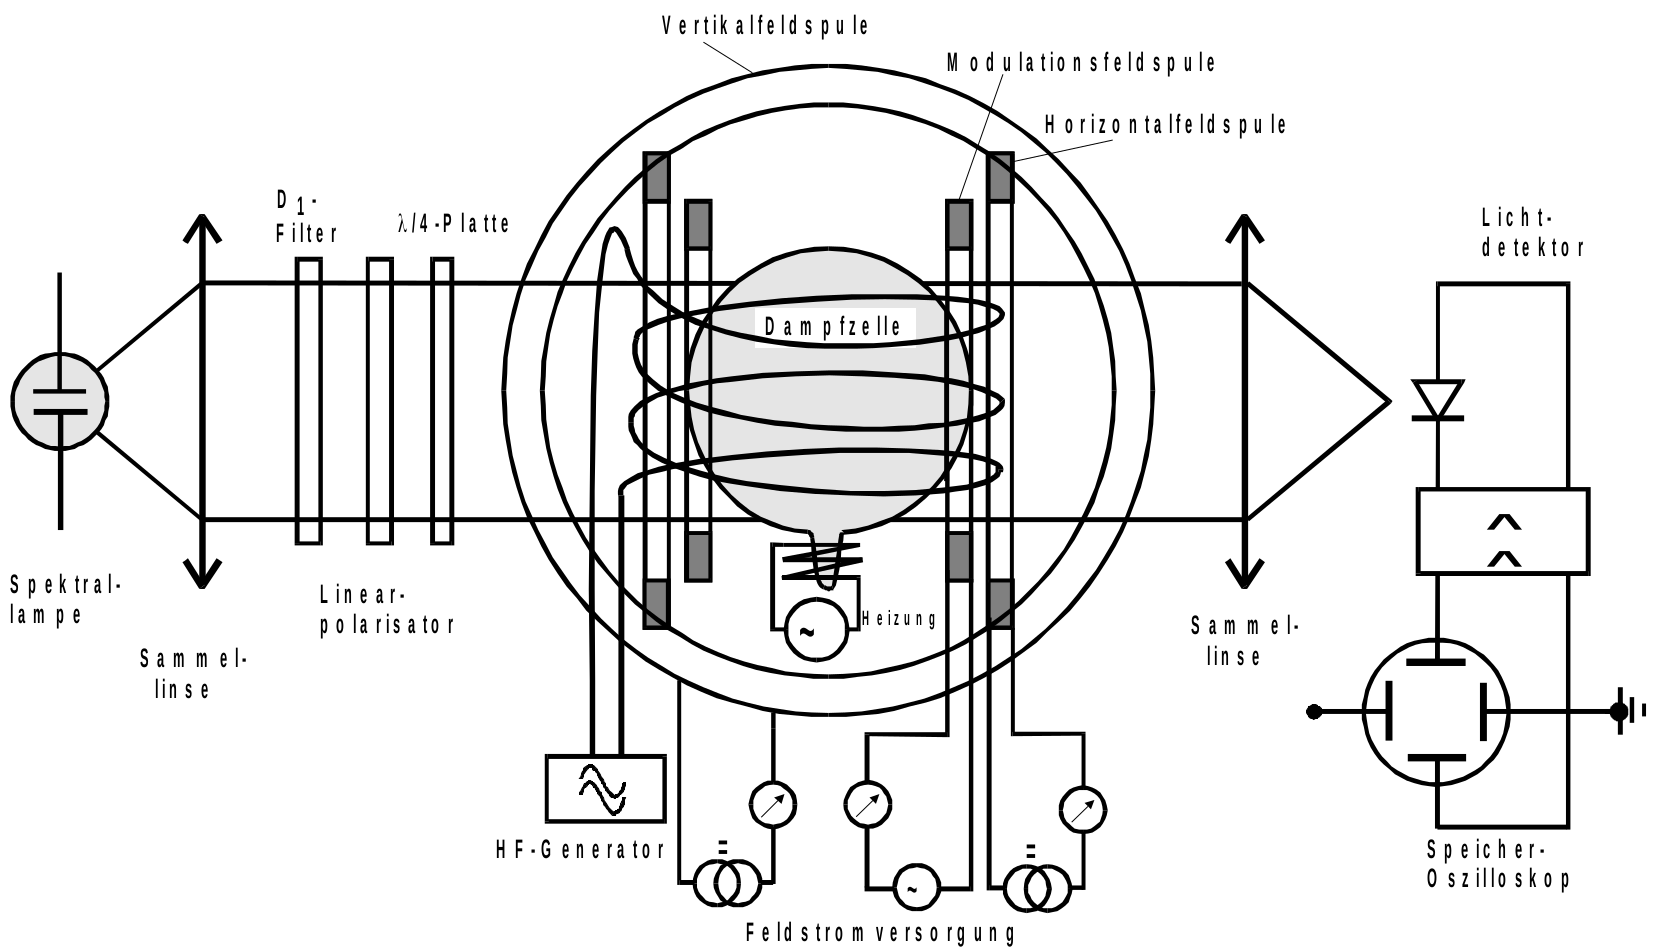
\includegraphics[keepaspectratio,width=0.8\textwidth]{content/images/aufbau.png}
\caption{Versuchsaufbau \cite{V21}.}
\label{fig:aufbau}
\end{figure}